\documentclass[aspectratio=169,11pt]{beamer}
\usepackage{fontspec}
\setsansfont{Segoe UI}
\usepackage{graphicx}
\definecolor{Forest}{HTML}{285D46}
\definecolor{Ink}{HTML}{17232D}
\definecolor{Muted}{HTML}{62717C}
\setbeamercolor{normal text}{fg=Ink,bg=white}
\setbeamercolor{frametitle}{fg=Forest}
\setbeamercolor{structure}{fg=Forest}
\setbeamerfont{frametitle}{size=\Large,series=\bfseries}
\setbeamertemplate{navigation symbols}{}
\setbeamertemplate{itemize item}{\small\textbullet}
\setbeamertemplate{footline}{\hfill\textcolor{Muted}{\scriptsize\insertframenumber\,/\,5}\hspace{5mm}\vspace{3mm}}
\setbeamersize{text margin left=8mm,text margin right=8mm}
\newcommand{\quiet}[1]{{\color{Muted}#1}}
\begin{document}

\begin{frame}[plain]
  \vspace{3mm}
  {\color{Forest}\fontsize{30}{35}\selectfont\bfseries Swallow Watch\par}
  \vspace{3mm}
  {\fontsize{19}{25}\selectfont A Lightweight Multimodal IoT\par Intrusion Detection System on ESP32\par}
  \vspace{7mm}
  {\large Detect nearby attacks.\par Observe device impact.\par Apply targeted repair and recovery.\par}
  \vfill
  \quiet{\small Yun-Xiang Lin \quad Yan-Wei Chen \quad Tzu-Hao Hsu\par
  National Sun Yat-sen University}
  \vspace{2mm}
\end{frame}

\begin{frame}{System architecture}
  {\large Wireless observations + local device state}
  \vspace{4mm}
  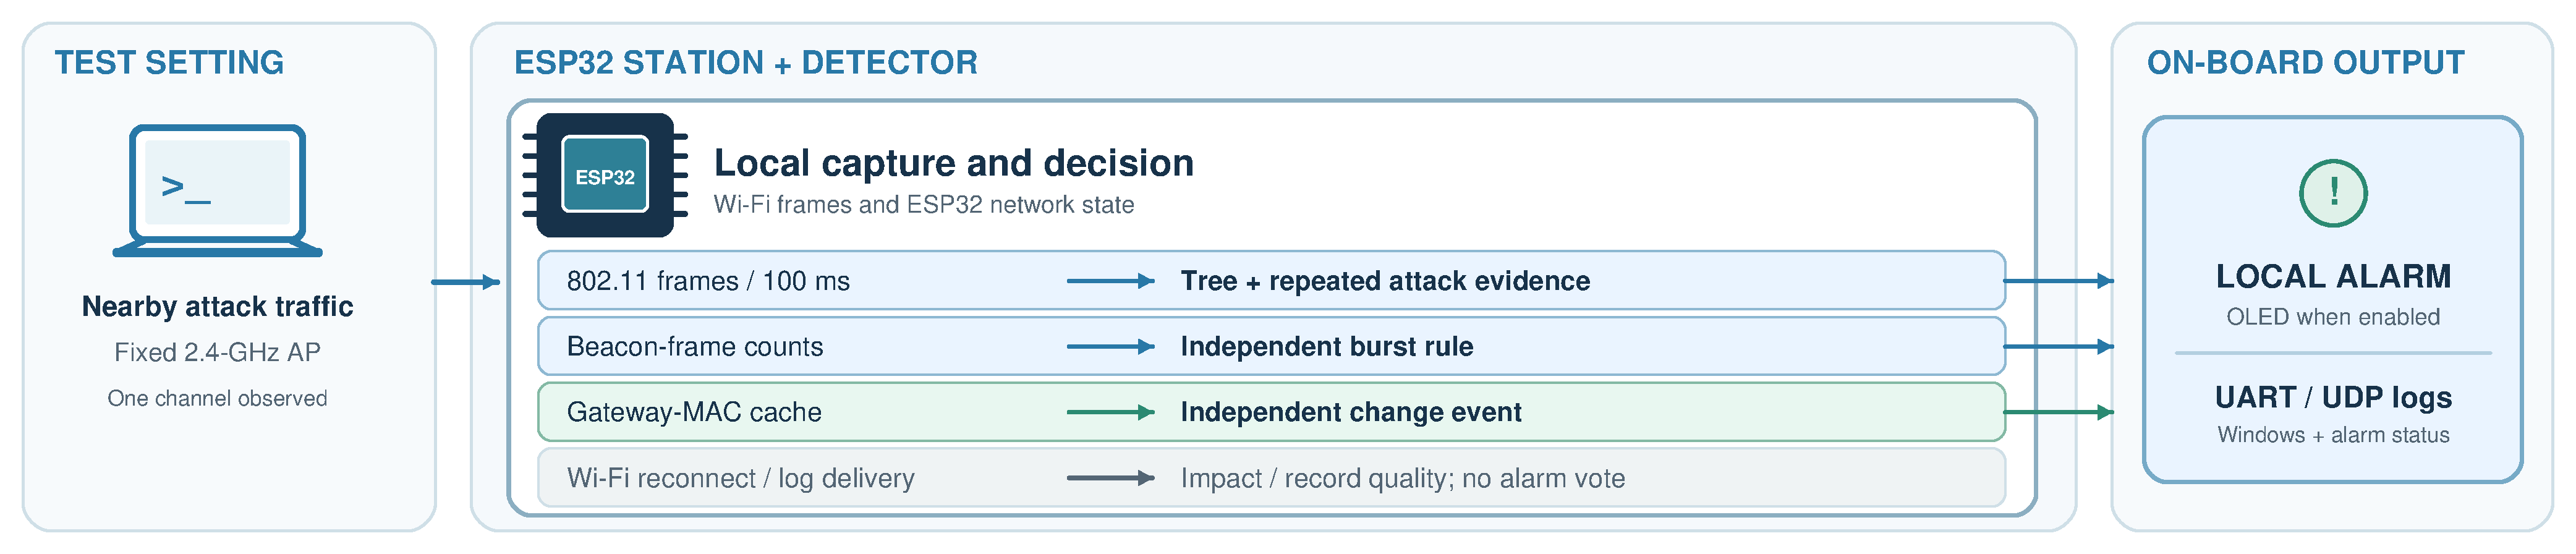
\includegraphics[width=\linewidth]{assets/system_architecture.pdf}
  \vspace{4mm}
  \begin{itemize}\setlength{\itemsep}{3mm}
    \item A compact tree and protocol rules run on the ESP32.
    \item Gateway identity adds ARP coverage; link state records impact.
    \item OLED and a live USB dashboard make decisions observable.
  \end{itemize}
\end{frame}

\begin{frame}{Fixed-AP detection results}
  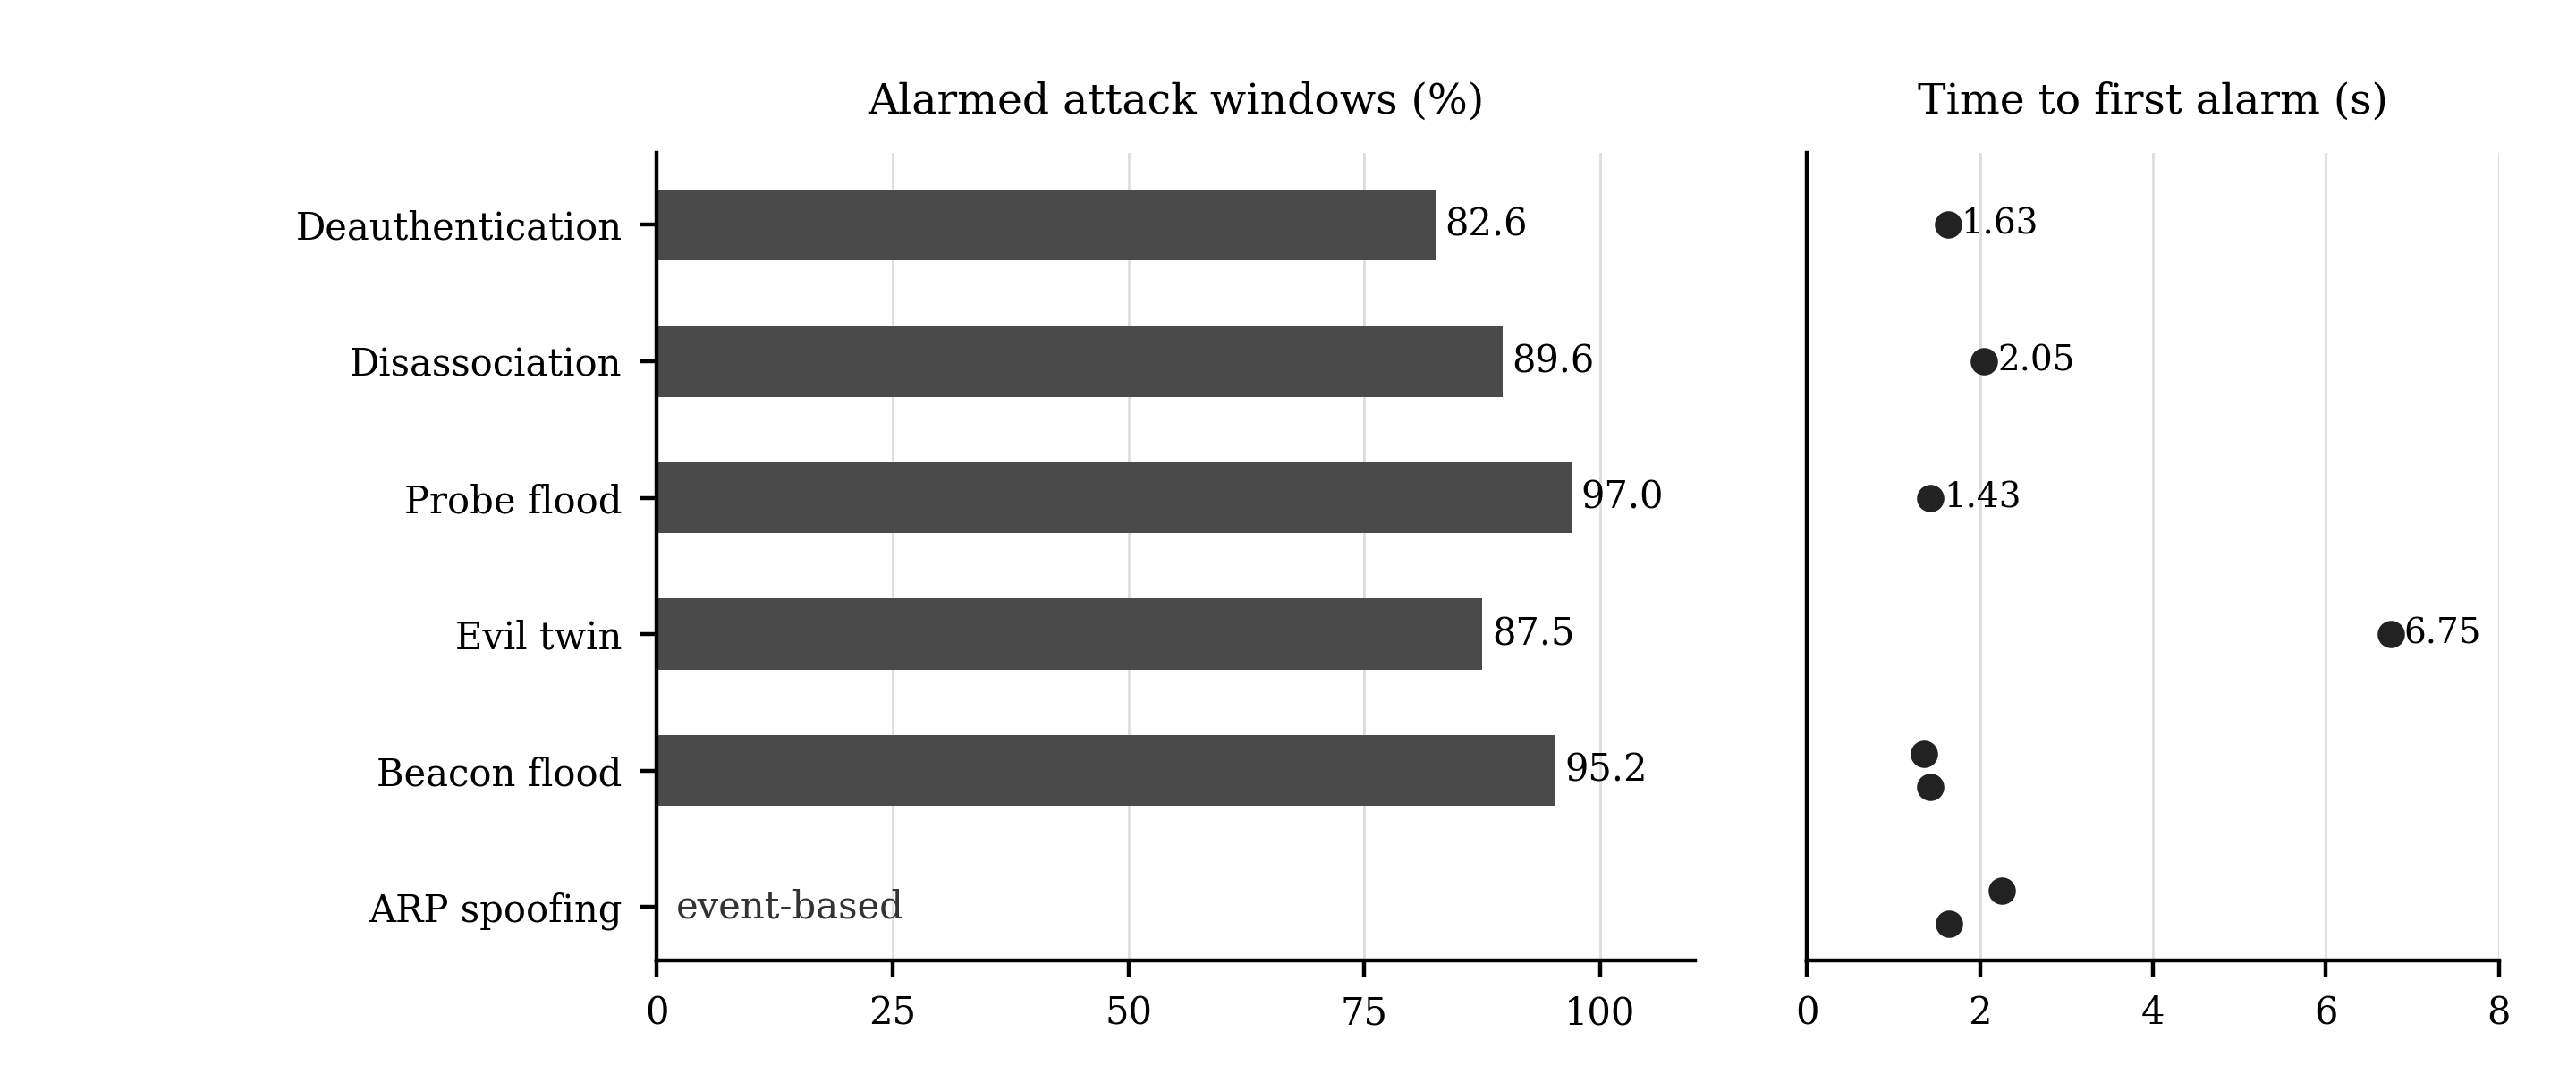
\includegraphics[width=\linewidth,height=5.55cm,keepaspectratio]{assets/detection_results.png}\par
  \vspace{1mm}
  {\small 8 attack runs across 6 scenarios; 1 false-alarm episode in 3 h 57 min.\par}
  \vspace{1mm}
  \quiet{\footnotesize Alarm coverage measures detection during an attack, not successful blocking.}
\end{frame}

\begin{frame}{Live demonstration}
  \begin{columns}[T,onlytextwidth]
    \begin{column}{.47\textwidth}
      {\Large\color{Forest}\bfseries ARP spoofing\par}
      \vspace{4mm}
      \begin{itemize}\setlength{\itemsep}{4mm}
        \item Detect gateway impersonation
        \item Repair and lock the trusted gateway
        \item Check actual router replies
      \end{itemize}
    \end{column}
    \begin{column}{.47\textwidth}
      {\Large\color{Forest}\bfseries Deauthentication\par}
      \vspace{4mm}
      \begin{itemize}\setlength{\itemsep}{4mm}
        \item Detect wireless attack traffic
        \item Observe a real Wi-Fi outage
        \item Reconnect and measure recovery
      \end{itemize}
    \end{column}
  \end{columns}
  \vspace{7mm}
  \quiet{\large Detection, protection, and recovery are separate outcomes.}
\end{frame}

\begin{frame}{Takeaways}
  \begin{itemize}\setlength{\itemsep}{6mm}
    \item \textbf{On-device detection:} six tested attack scenarios on a single AP.
    \item \textbf{Complementary sources:} wireless frames reveal attacks; host events add ARP coverage and endpoint context.
    \item \textbf{Visible response:} one-way ARP repair and automatic Wi-Fi recovery.
  \end{itemize}
  \vspace{6mm}
  \quiet{\small Two-way ARP remains unresolved. PMF is not enabled in this AP configuration.}
\end{frame}

\end{document}
